% Dorien Villafranco
% ME 721: Acoustic Bubble Dynamics
% Assignment #1
% 10/04/2016

\documentclass[12pt]{article}
\usepackage{geometry}
\usepackage{amsmath}
\usepackage{amssymb}
\usepackage{enumitem}
\usepackage{fancyhdr}
\usepackage{tikz}
\usetikzlibrary{trees}
\pagestyle{fancy}
\usepackage{amsmath}
\usepackage{listings}
\usepackage{caption}

\usepackage{color}
 
\definecolor{codegreen}{rgb}{0,0.6,0}
\definecolor{codegray}{rgb}{0.5,0.5,0.5}
\definecolor{codepurple}{rgb}{0.58,0,0.82}
\definecolor{backcolour}{rgb}{0.95,0.95,0.92}
 
\lstdefinestyle{mystyle}{
    backgroundcolor=\color{backcolour},   
    commentstyle=\color{codegreen},
    keywordstyle=\color{magenta},
    numberstyle=\tiny\color{codegray},
    stringstyle=\color{codepurple},
    basicstyle=\footnotesize,
    breakatwhitespace=false,         
    breaklines=true,                 
    captionpos=b,                    
    keepspaces=true,                 
    numbers=left,                    
    numbersep=5pt,                  
    showspaces=false,                
    showstringspaces=false,
    showtabs=false,                  
    tabsize=2}
\lstset{style=mystyle}

%\lhead{Problem \arabic{enumi}}
\lhead{Dorien Villafranco}
\chead{HW \#1}
\rhead{ME 721}

\begin{document}
\begin{enumerate}

% Problem 1
\item Code a numerical solution to the RP equation (1).\\
\noindent\rule{14cm}{0.4pt}\\
MATLAB was used to generate a solution to the Rayleigh-Plesset Equation. Variables were re-defined such that $y_1$ = R and $y_2$ = $\dot{R}$. This allowed the single 2nd order ODE to become 2 coupled $1^{st}$ order ODEs. Redefinition of variables resulted in:
\begin{align*}
\dot{y_1} = y_2  \qquad \dot{y_2} = \ddot{R}
\end{align*}
with
\begin{align*}
\ddot{R} = \Bigg[\frac{P(R,\dot{R},t)}{\rho} - \frac{3}{2}\dot{R}^2\Bigg]\frac{1}{R}
\end{align*}
where
\begin{align*}
P(R,\dot{R},t) = P_g^e\Bigg(\frac{R_o}{R}\Bigg)^{3k} + P_v - P_{\infty} - \frac{2\sigma}{R} - \frac{4\mu\dot{R}}{R}
\end{align*}
\begin{align*}
P_g^e = P_{\infty}^e - P_v + \frac{2\sigma}{R_o}
\end{align*}
\begin{align*}
P_\infty = P_\infty^e + P_a sin(\omega t)
\end{align*}
Shown below are the codes used to obtain solutions to the RP equation
\lstinputlisting[language=MATLAB]{HW1.m}
\lstinputlisting[language=MATLAB]{Rayleigh.m}

% Problem 2
\newpage
\item Perform the following sanity checks on your code:\\
\noindent\rule{14cm}{0.4pt}\\
i. Equilibrium: Set $P_a$ = 0; $\dot{R}$(t=0) = 0; R(t=0) = $R_o$ and run the code with these initial conditions for at least t = 0.001s. Plot R(t); is it stable? 
\begin{figure}[h]
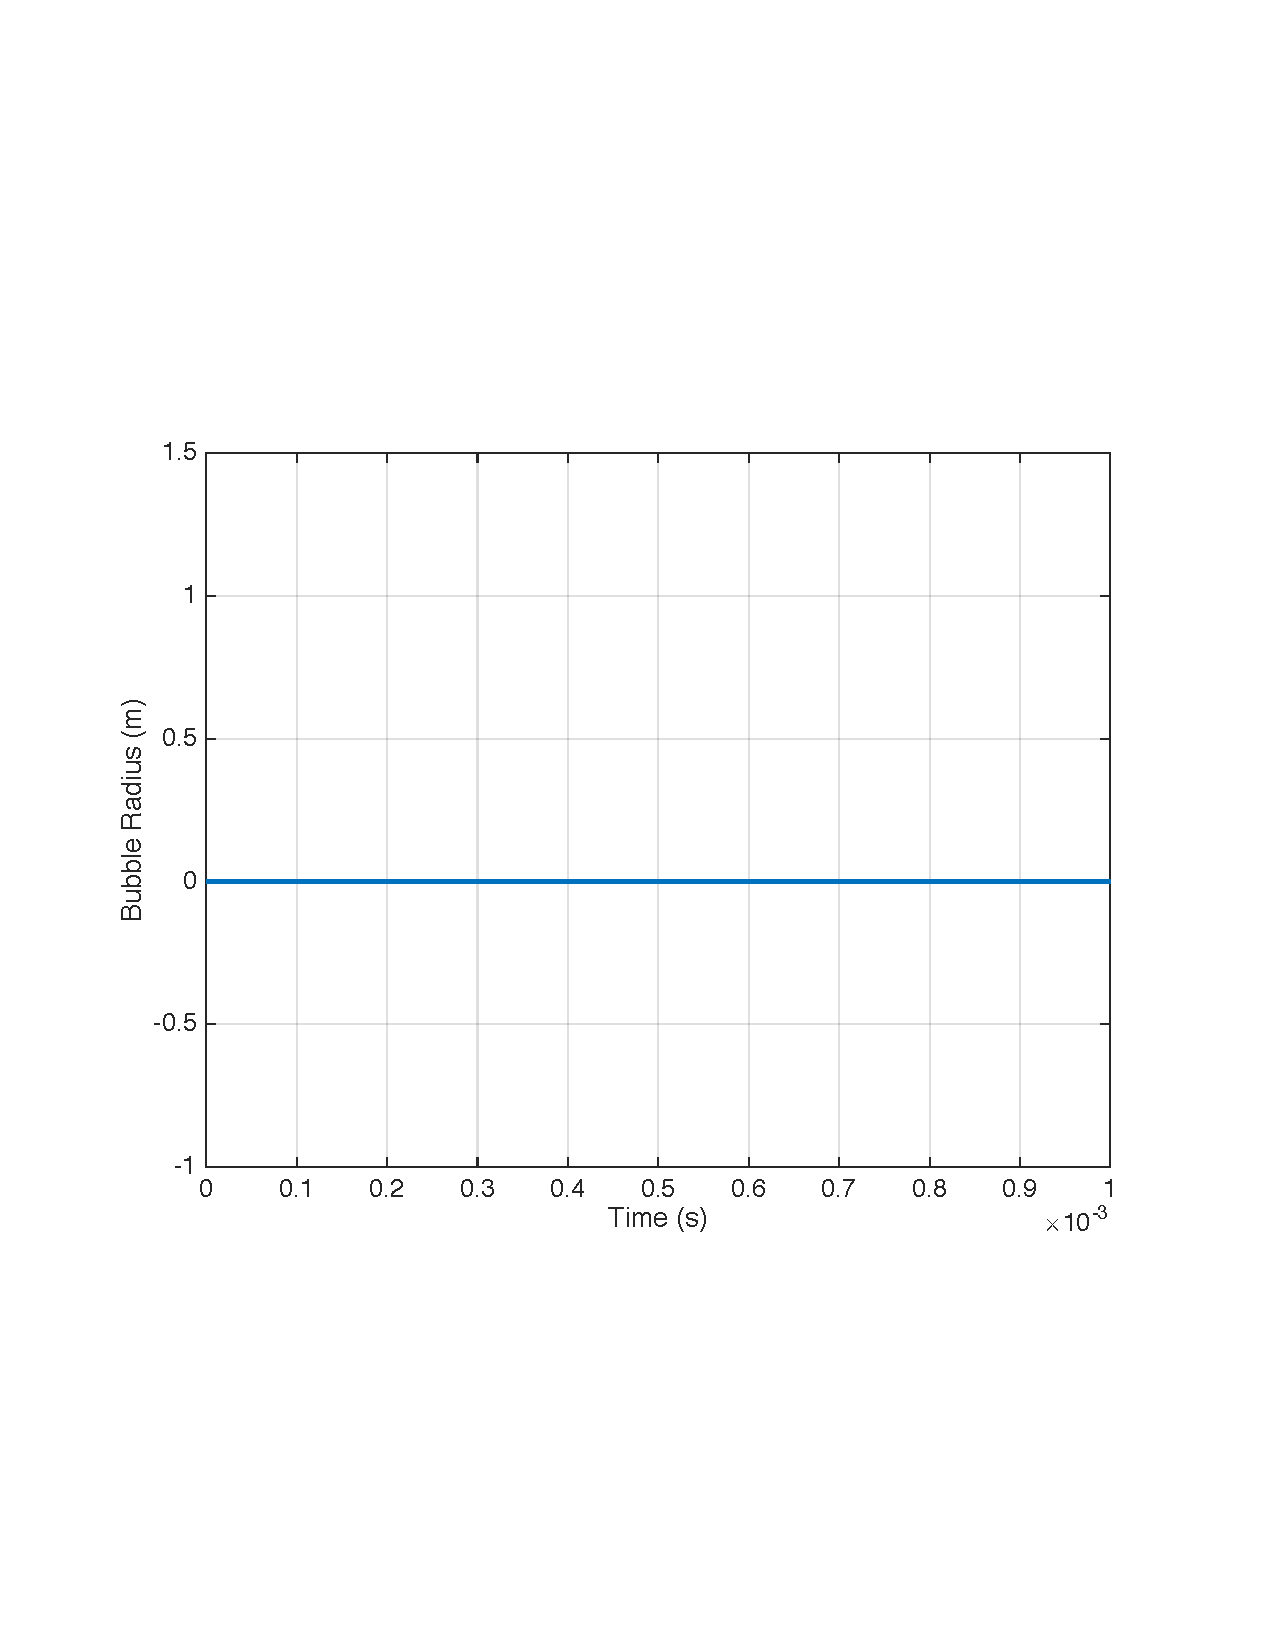
\includegraphics[scale = 0.4]{Fig_1}
\centering
\caption{Equilibrium Solution for the Rayleigh Plesset Equation}
\end{figure}

ii. Ring down:  Set run your code for each initial condition.  Plot R(t) does it decay to R0? What is the frequency of the ringing?  How does it compare with the linear natural frequency.
\begin{figure}[h]
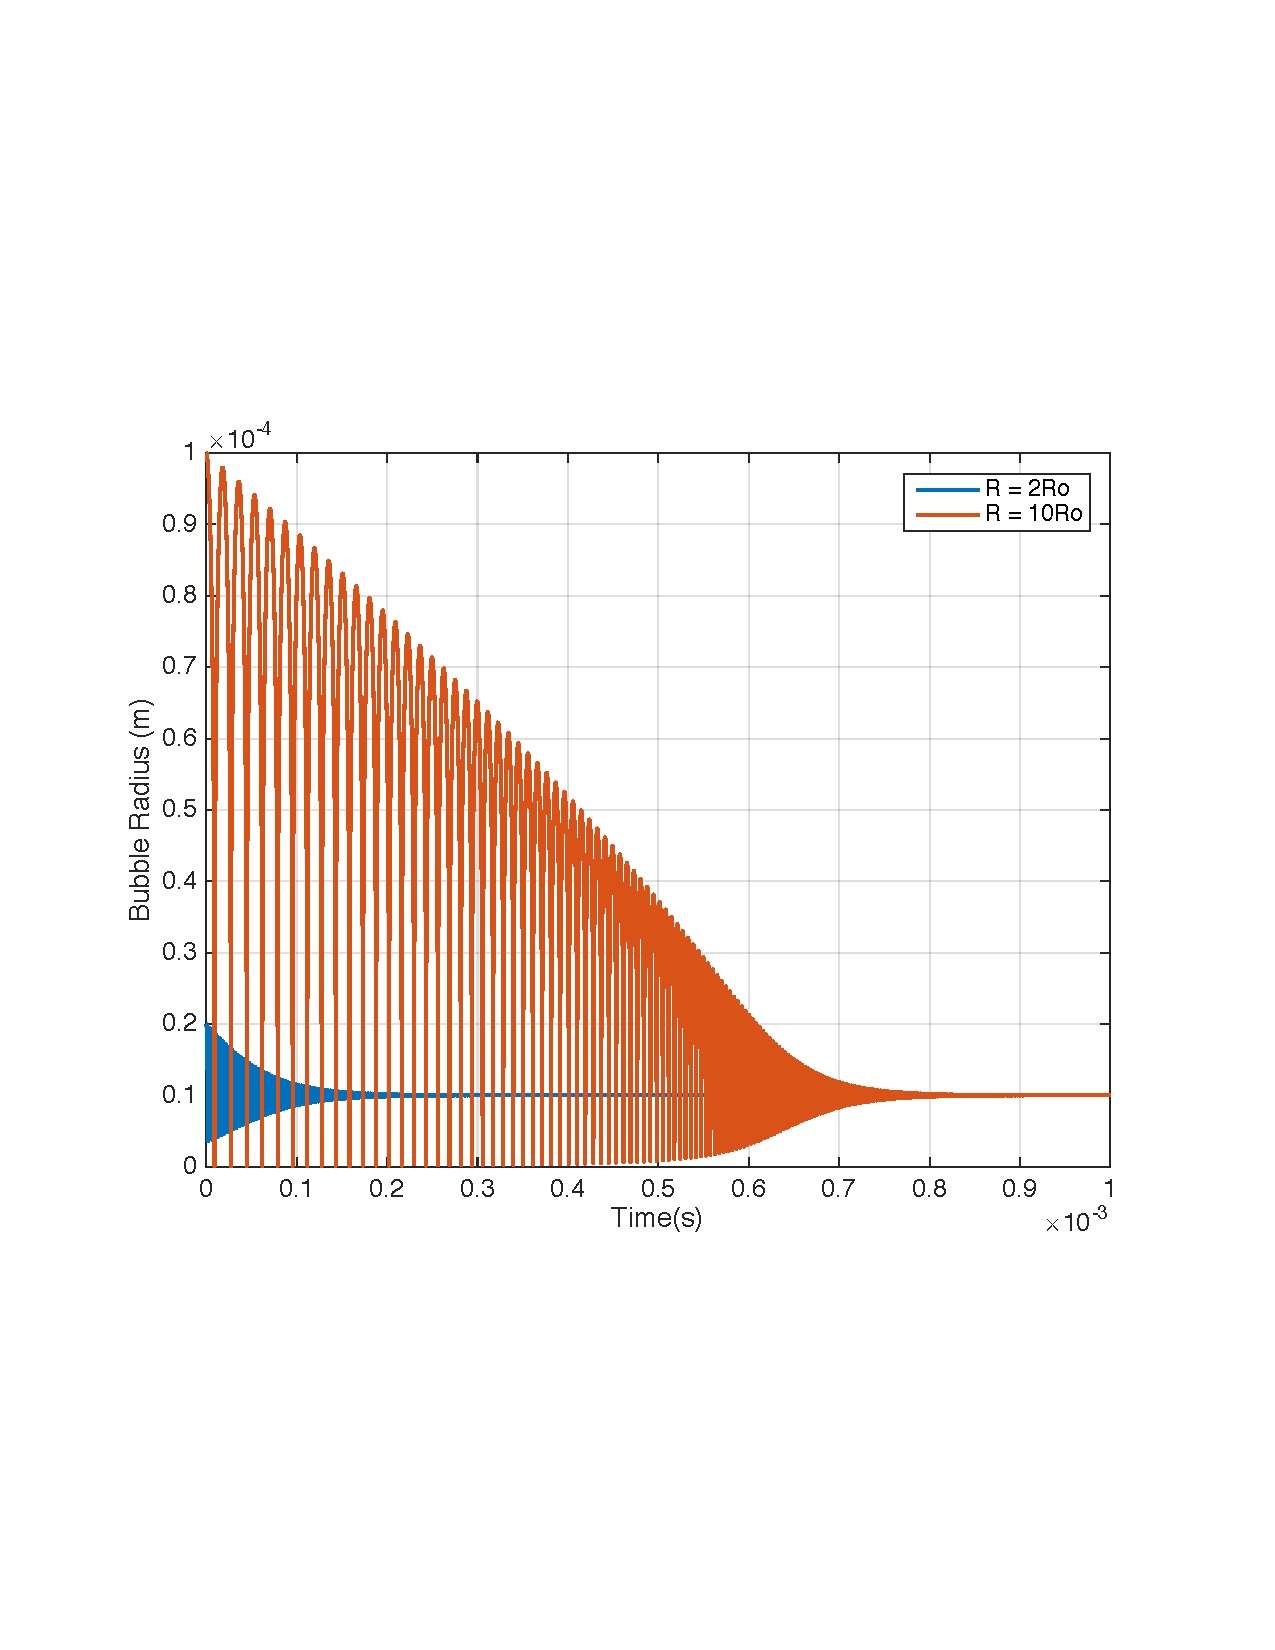
\includegraphics[scale = 0.4]{ring_down}
\centering
\caption{Ring Down test for Rayleigh Plesset Code}
\end{figure}

iii. Step drive: Set $\dot{R}$(t=0) = 0; R(t=0) = $R_0$; $P_{\infty}$ = $P^e_\infty$ + $P_cH(t-t_o)$ where $P_c$ is 1x$10^5$ Pa and H(t) is the unit step function (Heaviside). Plot R(t) does it make sense? 
\begin{figure}[h]
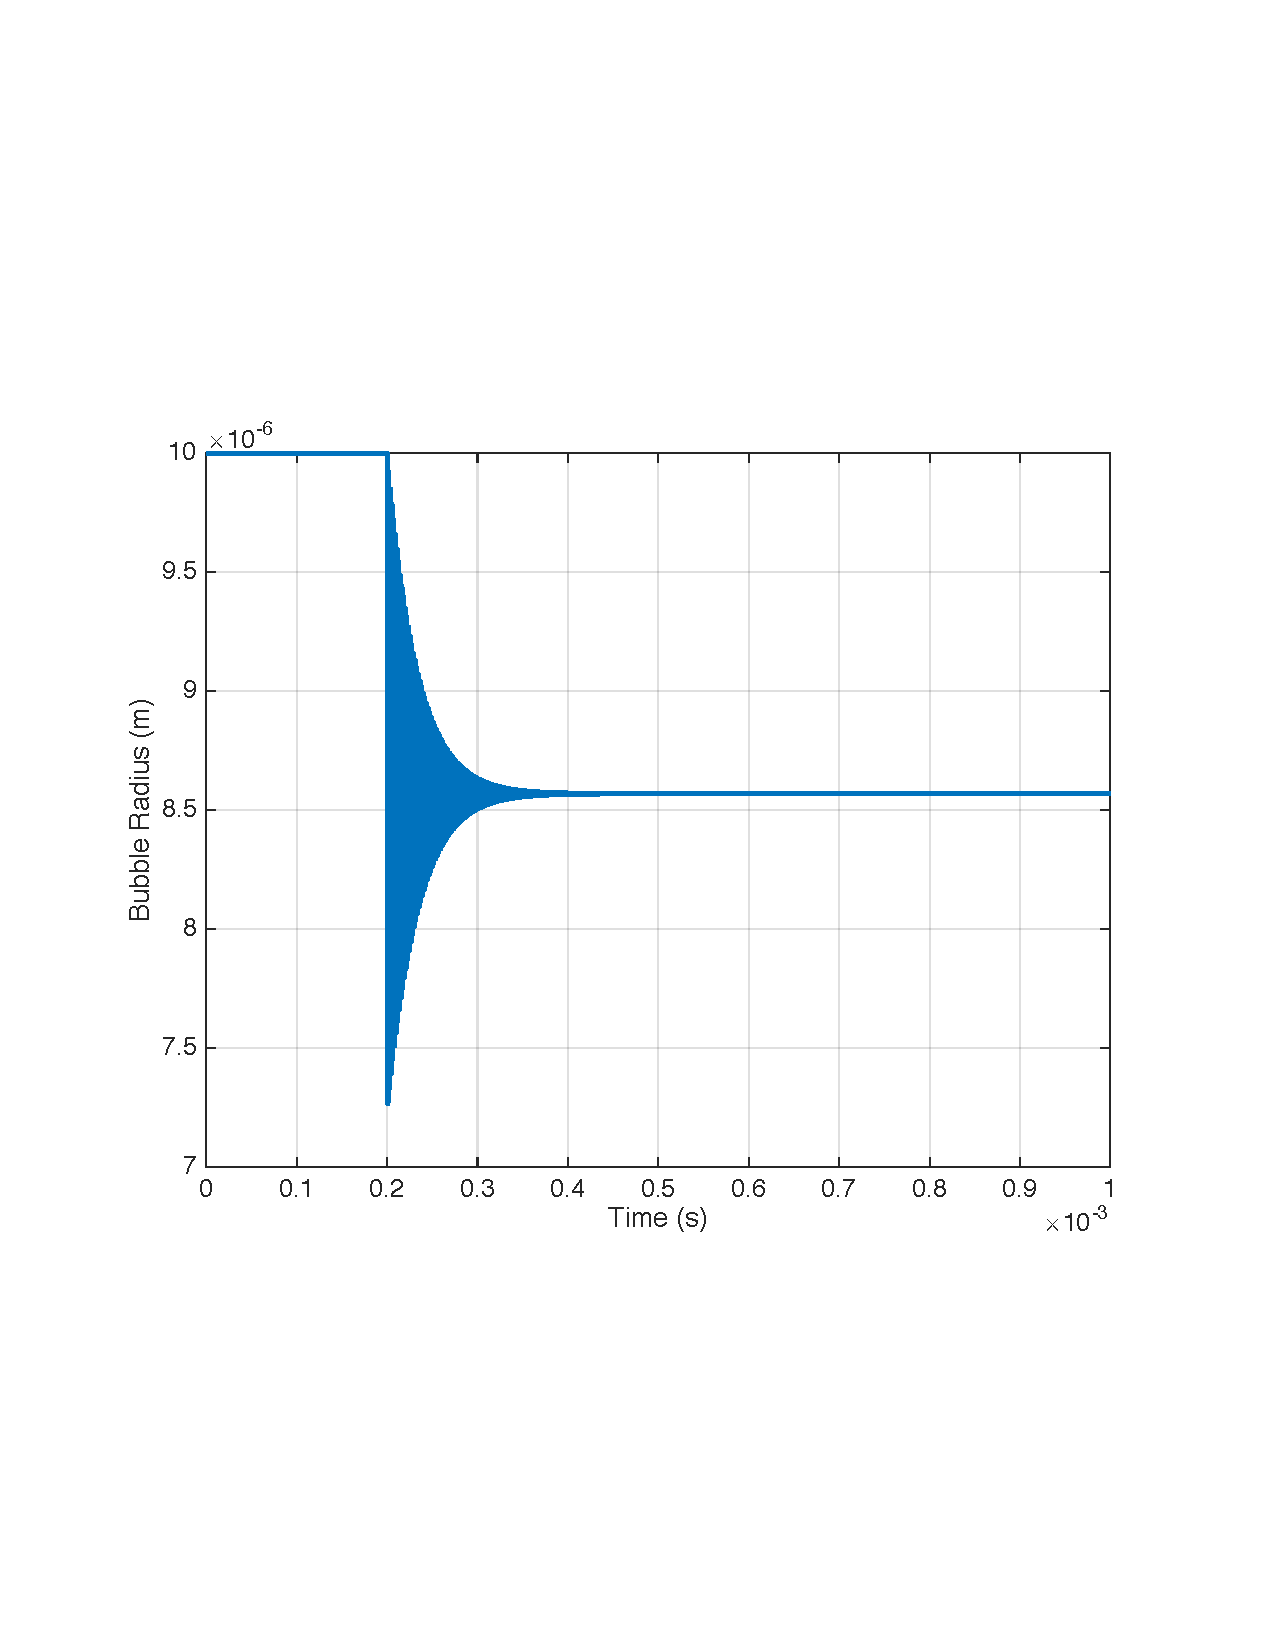
\includegraphics[scale = 0.4]{Step_Test}
\centering
\caption{Step Drive test for Rayleigh Plesset Code}
\end{figure}

% Problem 3
\newpage
\item Benchmark your code against a previously published solution, using their parameter values.  You may choose anything nontrivial* in the literature of the past 50 years, but be careful to compare results of the same equation at the same parameters, since there are a variety of Rayleigh-Plesset equations.
\noindent\rule{14cm}{0.4pt}\\
I used the parameters laid out in the paper by Lauterborn. The figure below shows the comparison of the results. Not sure why they do not align properly. It may be an incorrect use of his parameters in the papers or a sign difference in the equation - will double check later and update. 

\begin{figure}[h]
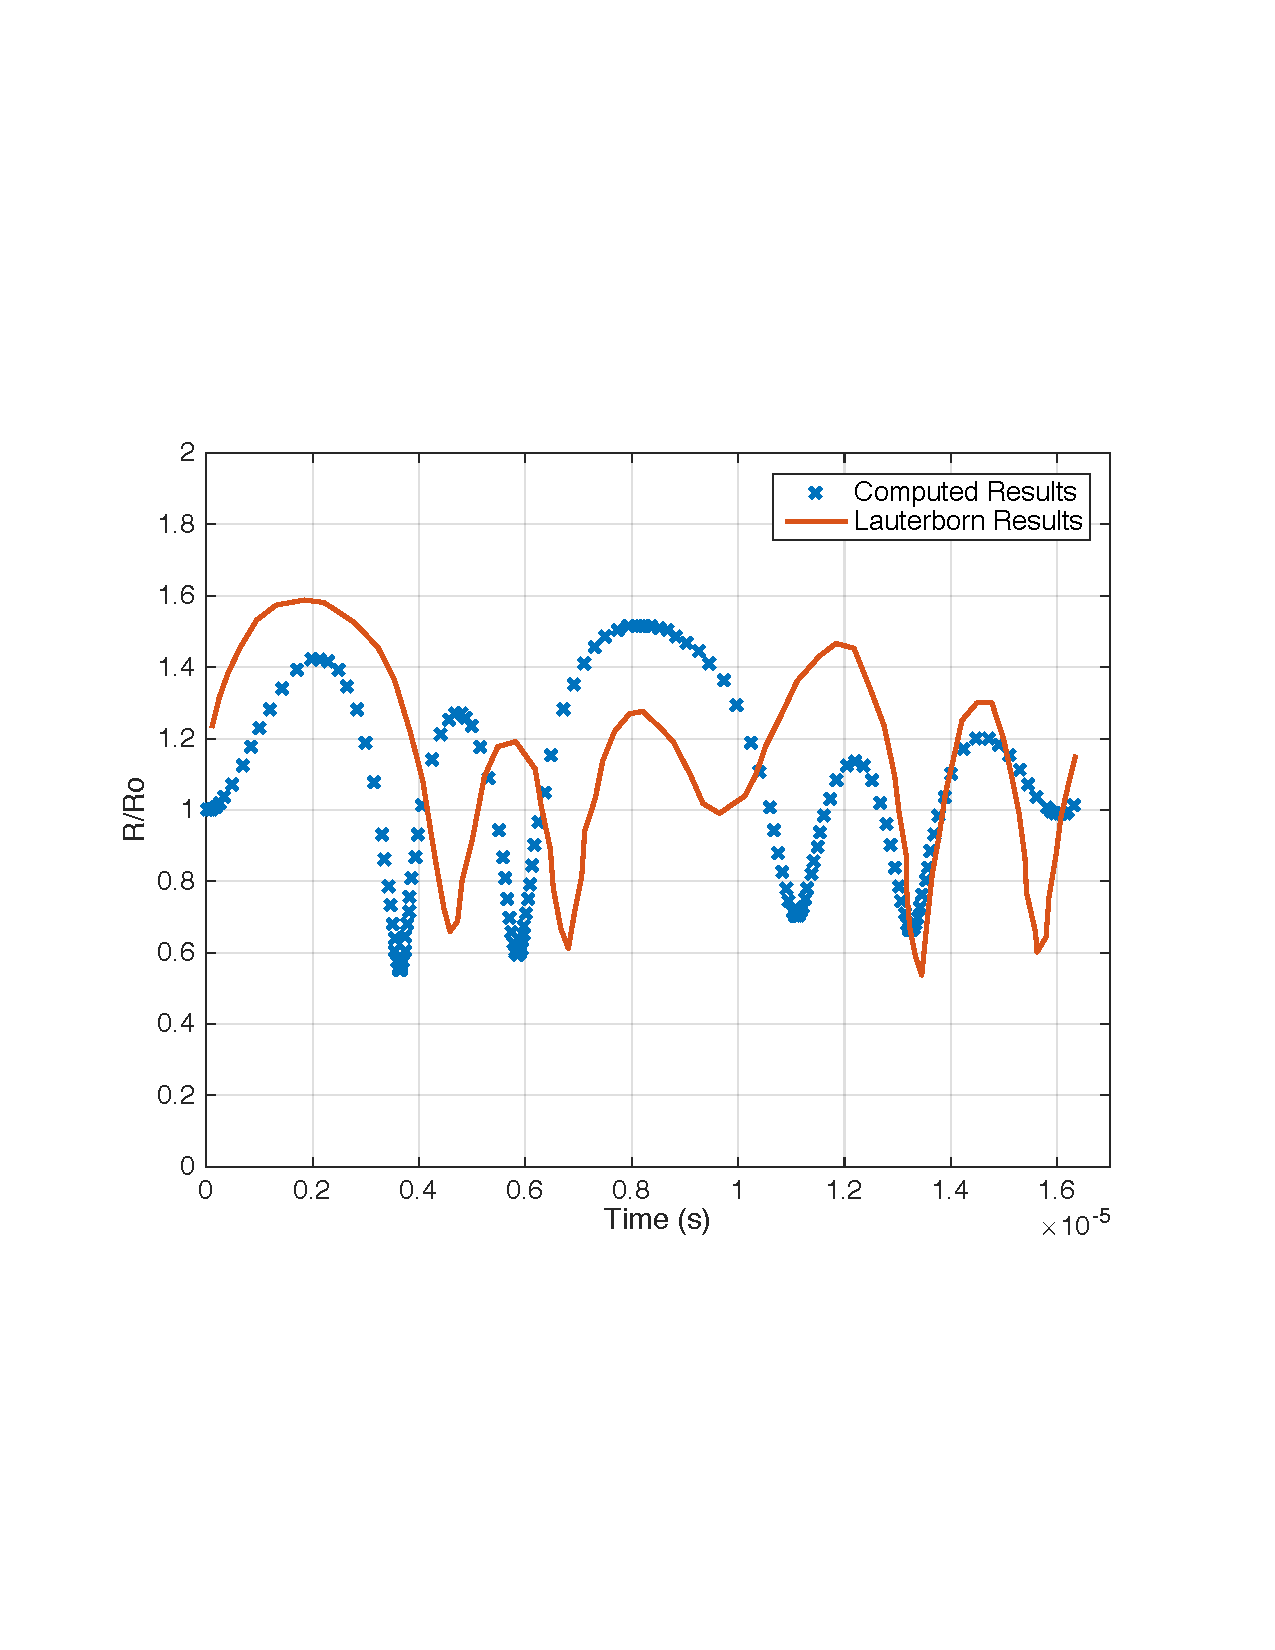
\includegraphics[scale = 0.4]{Lauterborn_Compare}
\centering
\caption{Comparison of Computational Results with those obtained by Lauterborn}
\end{figure}

% Problem 4
\newpage
\item Recall the linear EOM we derived in class for R(t) = $R_o$ + y(t), y $<<$ $R_o$
\begin{align*}
\ddot{y} + \Bigg(\frac{4\mu}{\rho R_o^2}\Bigg)\dot{y} + \frac{1}{\rho R_o^2}\Bigg(3k\Bigg(P_\infty^e - P_v + \frac{2\sigma}{R_o}\Bigg) - \frac{2\sigma}{R_o}\Bigg)y = \frac{-P}{\rho R_o}sin(\omega t)
\end{align*}
\noindent\rule{14cm}{0.4pt}\\
i. Code a numerical integration solution to (3)
\lstinputlisting[language=MATLAB]{Runge_Kutta.m}

ii. Benchmarks 
Works for all similar cases. See comparison in Problem 5


% Problem 5
\newpage 
\item For the linearized EOM in problem 4, we can approximate the natural frequency as:
\begin{align*}
\omega_o^2 = \frac{3kP_\infty^e}{\rho R_o^2}
\end{align*}
and the damping ratio as:
\begin{align*}
\xi = \frac{2\mu}{(\rho R_o^2 3kP_\infty^2)^{0.5}}
\end{align*}
with the usual solution to sine forcing given as:
\begin{align*}
y(t) = \frac{-P_a}{\rho R_o \omega_o^2} M(\omega) sin(\omega t + \phi(\omega))
\end{align*}
\noindent\rule{14cm}{0.4pt}\\
i. Compare results of all there developments of R(t)
\begin{figure}[h]
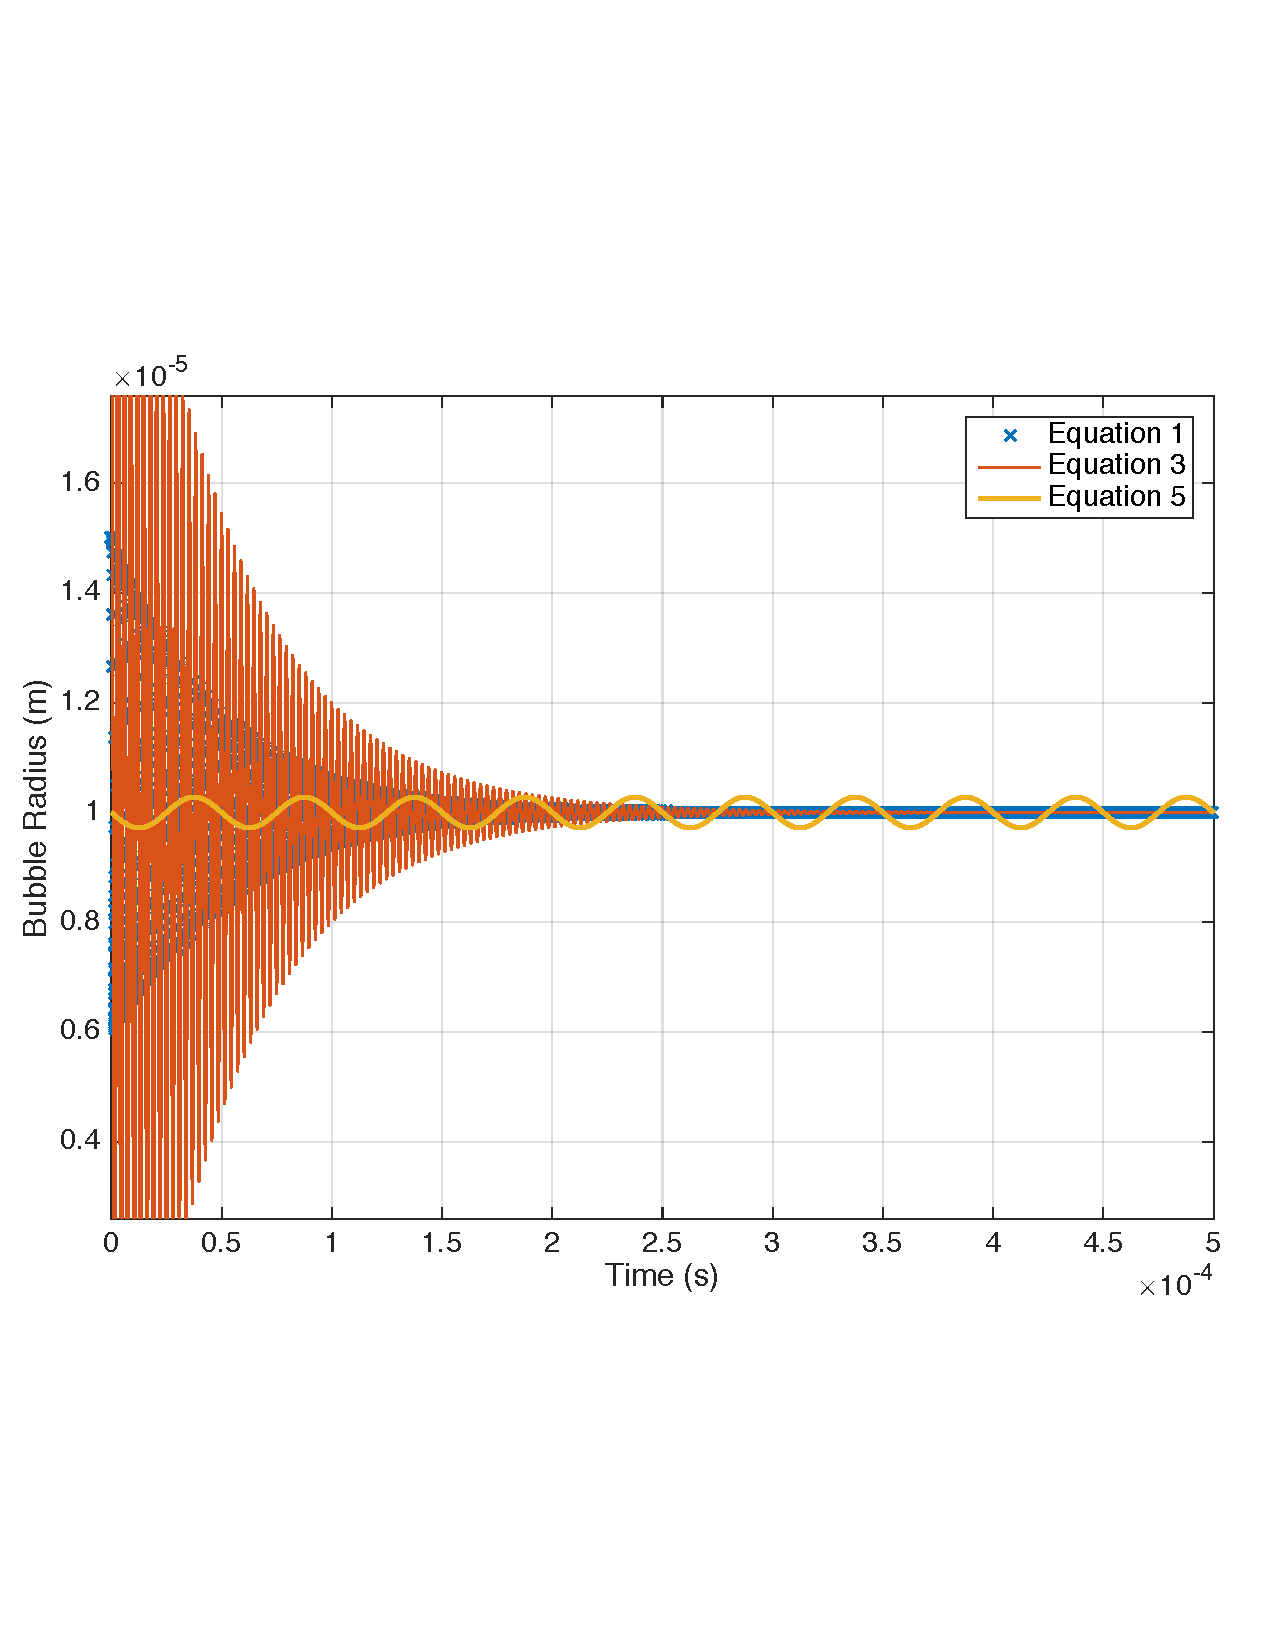
\includegraphics[scale = 0.5]{Compare_All}
\centering
\caption{Comparison of all developments of R(t)}
\end{figure}
\end{enumerate}
\end{document}